\documentclass[10pt]{article}
\usepackage[russian]{babel}
\usepackage[utf8]{inputenc}
\usepackage[T2A]{fontenc}
\usepackage{amsmath}
\usepackage{amsfonts}
\usepackage{amssymb}
\usepackage[version=4]{mhchem}
\usepackage{stmaryrd}
\usepackage{graphicx}
\usepackage[export]{adjustbox}
\graphicspath{ {./images/} }

%New command to display footnote whose markers will always be hidden
\let\svthefootnote\thefootnote
\newcommand\blfootnotetext[1]{%
  \let\thefootnote\relax\footnote{#1}%
  \addtocounter{footnote}{-1}%
  \let\thefootnote\svthefootnote%
}

%Overriding the \footnotetext command to hide the marker if its value is `0`
\let\svfootnotetext\footnotetext
\renewcommand\footnotetext[2][?]{%
  \if\relax#1\relax%
    \ifnum\value{footnote}=0\blfootnotetext{#2}\else\svfootnotetext{#2}\fi%
  \else%
    \if?#1\ifnum\value{footnote}=0\blfootnotetext{#2}\else\svfootnotetext{#2}\fi%
    \else\svfootnotetext[#1]{#2}\fi%
  \fi
}

\begin{document}
\section*{Параметрические колебания нелинейных систем}
Параметрический резонанс и параметрическая неустойчивость в линейной системе

Специфическим видом внешнего воздействия на колебательную систему является периодическое изменение параметров системы во времени. Такое воздействие называется параметрическим. Начнем с краткого напоминания об основных особенностях параметрических колебаний в линейных системах ${ }^{1}$.

Рассмотрим простую модельную систему: колебательный контур с переменной емкостью (рис. 16.1). Изменение емкости со временем можно обеспечить, например, механически изменяя расстояние между пластинами конденсатора. В таком случае мгновенные значения заряда $q$ и напряжения $u$ на емкости будут связаны соотношением $q(t)=C(t) u(t)$. Это позволяет записать дифференциальное уравнение, описывающее колебания в контуре


\begin{equation*}
\ddot{q}+\frac{1}{L C(t)} q=0 \tag{16.1}
\end{equation*}


Уравнение (16.1) имеет вид уравнения гармонического осциллятора, собственная частота которого зависит от времени.\\
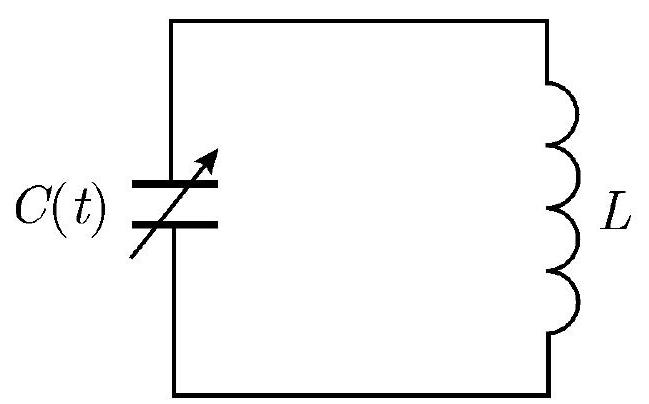
\includegraphics[max width=\textwidth, center]{2024_12_13_864dea76193ac5d12698g-258}

Рис. 16.1. Колебательный контур с переменной емкостью\\
Пусть емкость конденсатора изменяется следующим образом. В моменты времени, когда заряд на конденсаторе максимален, пластины резко раздвигаются. При

\footnotetext{${ }^{1}$ Параметрические колебания в линейных системах и явление параметрического резонанса достаточно подробно обсуждаются в книге «Линейные колебания и волны», входящей в состав настоящей серии.
}этом емкость уменьшается от некоторого значения $C_{2}$ до значения $C_{1}<C_{2}$. Поскольку заряд на конденсаторе при этом не изменяется, напряжение скачком возрастет от значения $V_{2}$ до значения $V_{1}=C_{2} V_{2} / C_{1}$. В моменты времени, когда заряд равен нулю, пластины так же резко сдвигаются; емкость при этом увеличивается, а напряжение остается равным нулю (рис. 16.2). В таком процессе постоянно совершается работа, которая идет на увеличение энергии колебаний. За один период приращение энергии составит (необходимо учесть, что в течение периода пластины раздвигаются дважды)


\begin{equation*}
\Delta W=2\left(W_{1}-W_{2}\right)=C_{1} V_{1}^{2}-C_{2} V_{2}^{2}=C_{2} V_{2}^{2}\left(\frac{C_{2}}{C_{1}}-1\right) \tag{16.2}
\end{equation*}


Если ввести обозначения $\Delta C=C_{2}-C_{1}, C=\left(C_{1}+C_{2}\right) / 2$ и считать, что $\Delta C \ll C$, соотношение (16.2) можно переписать в виде


\begin{equation*}
\Delta W \approx 2 W \frac{\Delta C}{C} . \tag{16.3}
\end{equation*}


\begin{center}
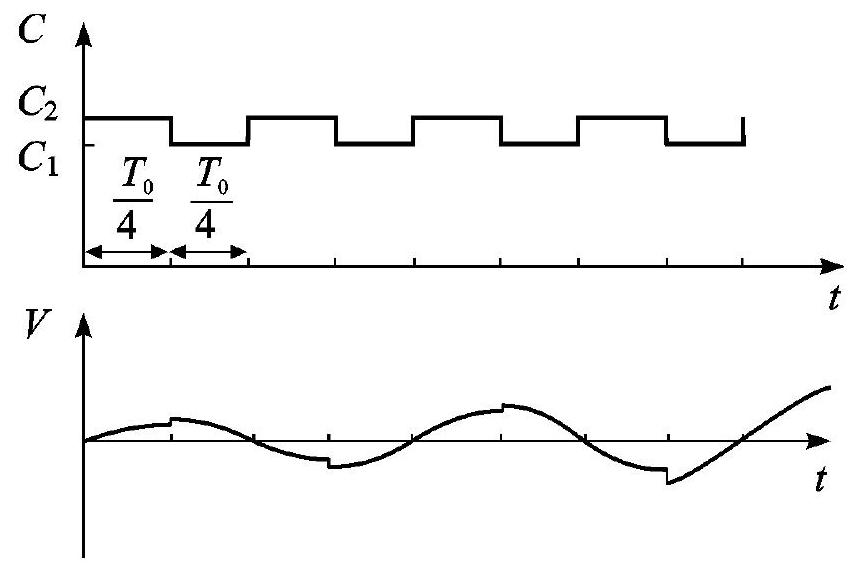
\includegraphics[max width=\textwidth]{2024_12_13_864dea76193ac5d12698g-259}
\end{center}

Рис. 16.2. Зависимость от времени емкости и напряжения в колебательном контуре с механически перестраиваемым конденсатором

Из приведенных выше рассуждений следует, что для эффективного поступления энергии в систему период колебаний $T_{0}$ и период изменения параметра $T$ должны быть связаны соотношением


\begin{equation*}
T \approx \frac{T_{0}}{2} \tag{16.4}
\end{equation*}


которое представляет собой условие параметрического резонанса. Отметим отличие от резонансного условия при вынужденных колебаниях линейного осциллятора, $T \approx T_{0}$.

Можно, однако, раздвигать пластины не каждый раз, когда заряд на конденсаторе максимален, а через раз; энергия все равно будет поступать в систему, хотя и в меньшем количестве. Более того, очевидно, что это можно делать в общем случае только в каждый $n$-ный благоприятный момент. Таким образом, имеется, вообще говоря, бесконечное число параметрических резонансов, условия которых имеют вид


\begin{equation*}
T \approx \frac{n T_{0}}{2} \tag{16.4}
\end{equation*}


Число $n=1,2, \ldots$ будем называть порядком резонанса, а резонанс при $n=1$ - основным.

При выполнении условий резонанса колебания в линейной системе, как можно видеть на рис. 16.2, неограниченно нарастают. Это явление называется параметрической неустойчивостью.

Основной моделью в теории параметрических колебаний в линейных системах служит уравнение Матьё


\begin{equation*}
\ddot{x}+\omega_{0}^{2}(1+f \cos \omega t) x=0, \tag{16.5}
\end{equation*}


которое представляет собой уравнение линейного осциллятора с гармоническим параметрическим возбуждением. Это уравнение детально исследовано математиками; более того, его решения составляют особый класс специальных функций - функции Матьё. Для наших дальнейших целей важно отметить следующие его свойства. На плоскости параметров амплитуда - частота воздействия существуют зоны неустойчивости, которые имеют вид характерных клювов, расположенных в окрестности резонансных частот


\begin{equation*}
\omega \approx \frac{2 \omega_{0}}{n} . \tag{16.6}
\end{equation*}


Перейдем к новой независимой переменной $\tau=\omega t / 2$. Тогда уравнение (16.5) можно переписать в виде


\begin{equation*}
x^{\prime \prime}+(a+2 q \cos 2 \tau) x=0 \tag{16.7}
\end{equation*}


где $a=4 \omega_{0}^{2} / \omega^{2}, q=2 \omega_{0}^{2} f / \omega^{2}$, штрихи обозначают дифференцирование по $\tau$. Зоны неустойчивости на плоскости параметров $(a, q)$ изображены на рис. 16.3. В новых переменных резонансное условие (16.6) принимает вид $a \approx n^{2}$.

Отметим следующие отличия от резонанса при вынужденных колебаниях. Вопервых, малая расстройка (в пределах зоны неустойчивости) не может стабилизировать неустойчивость, тогда как при вынужденных колебаниях амплитуда нарастает до бесконечности только в случае точного резонанса $\omega=\omega_{0}$. Кроме того нарастание амплитуды параметрических колебаний происходит по экспоненйильному закону, а не по линейному.\\
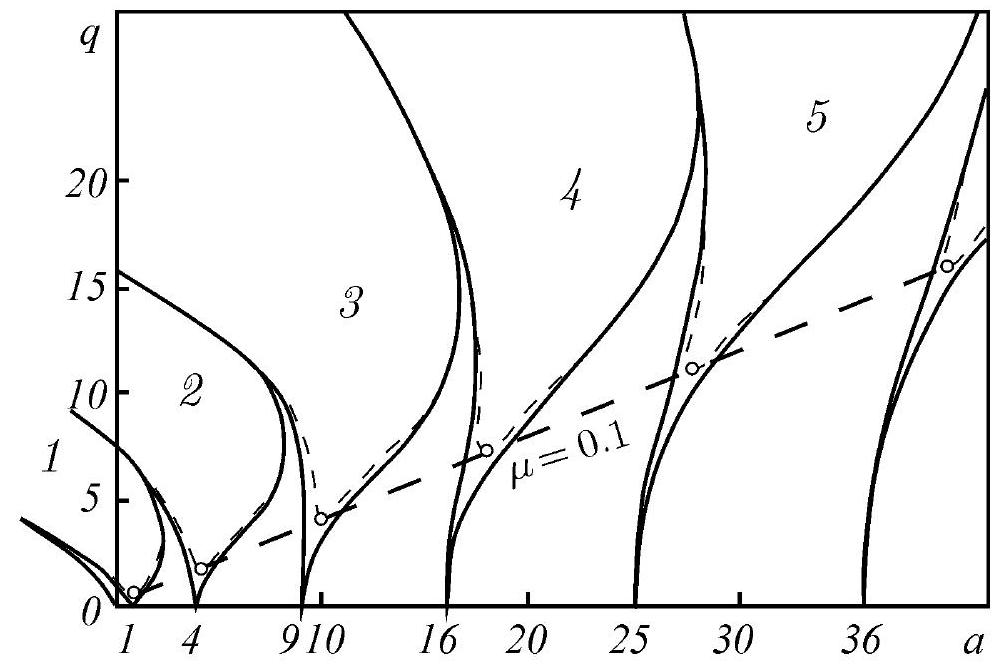
\includegraphics[max width=\textwidth, center]{2024_12_13_864dea76193ac5d12698g-261}

Рис. 16.3. Границы зон неустойчивости на плоскости параметров $(a, q)$ для уравнения Матьё. Цифры l-5 соответствуют номерам резонансов.

Добавление линейного затухания также не стабилизирует неустойчивость, а лишь сужает границы зон (на рис. 16.3 они показаны штриховой линией). Действительно, если рассмотреть уравнение параметрического осциллятора с затуханием


\begin{equation*}
y^{\prime \prime}+2 \gamma y^{\prime}+(b+2 q \cos 2 \tau) x=0, \tag{16.8}
\end{equation*}


нетрудно показать, что заменой $y=x \exp [-\gamma \tau]$ оно может быть приведено к виду (16.7), где $a=b-\gamma^{2}$. Чтобы решение уравнения (16.8) было неустойчивым, необходимо, чтобы соответствующее решение уравнения (16.7) нарастало как $\exp (p \tau)$, где $p>\gamma$. Поэтому границы зон неустойчивости сдвигаются вверх. Поскольку амплитуда воздействия должна превышать некоторое пороговое значение (которое увеличивается с ростом номера резонанса), говорят, что неустойчивость носит пороговый характер.

Отсюда следует, что нелинейность играет принципиальную роль в теории параметрических колебаний. Только учет нелинейных эффектов позволяет ответить на вопрос, чем заканчивается развитие неустойчивости на больших временах, и определить характеристики установившегося режима колебаний. Аналогичная ситуация имеет место и для автоколебаний (лекция 11).


\end{document}